%%%% CS 383 HW #7 - team3-hw7.tex
%%%% Due on BBLearn before 10pm on Monday 4/25/2016


%##########################################################################################################################################################################
% Header
%##########################################################################################################################################################################

\documentclass[11pt]{report}

\usepackage{graphicx}
\usepackage{caption}
\usepackage{hyperref}

\marginparwidth 0.5in 
\oddsidemargin 0.25in 
\evensidemargin 0.25in 
\marginparsep 0.25in
\topmargin 0.0in 
\textwidth 6in \textheight 8.5in

\title{Sprint Report \#7 for Team Lambda}
\author{jank6275, mora5651, boss2849, bolt1003, gall7417, brec9824, snev7821, mars2681}

\begin{document}

\maketitle

\tableofcontents
\chapter{Links}
    Our source code can be found at \url{https://github.com/uidaho/squireproject}, the issue tracker and backlog can be found at \url{https://github.com/uidaho/squireproject/issue}, and our documentation can be found at \url{https://github.com/uidaho/squireproject/wiki}.

\chapter{Implemented Use Cases}
\section{General}
    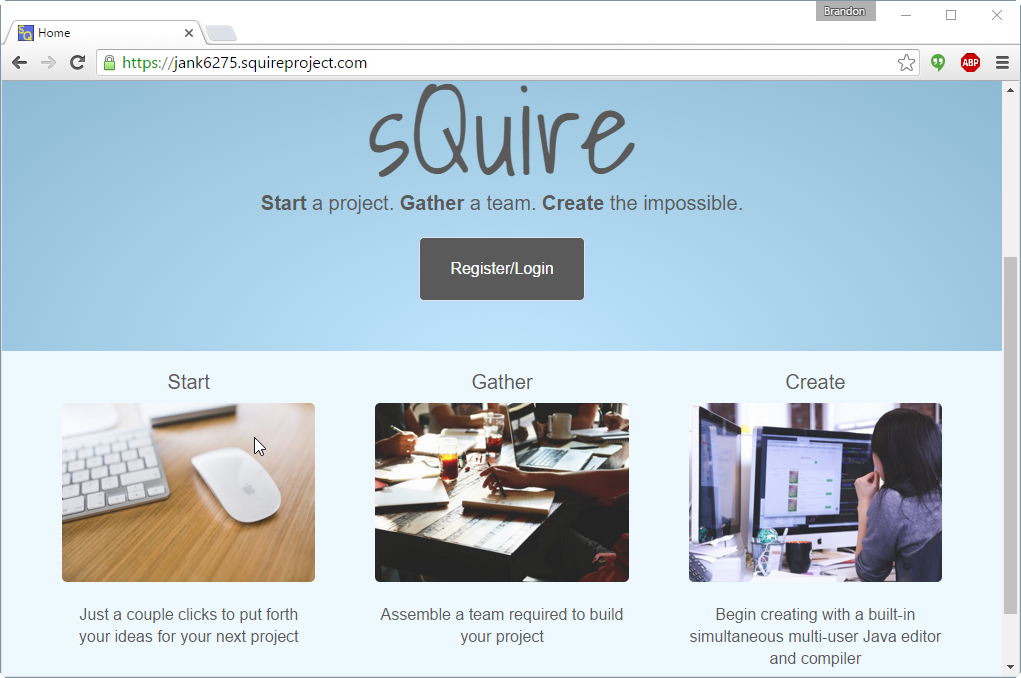
\includegraphics[width=0.9\textwidth]{images/index}
    \begin{itemize}
        \item The project was migrated to use bootstrap CSS, creating a clean and unified look for the project. (jank6275)
        \item Modified site to be a fully responsive layout. Users can use any modern browser on any device, including apple and android devices. (jank6275)
        \item Added 403 page (forbidden access). (brec9824)
    \end{itemize}
    
\section{Editor Team (jank6275)}
    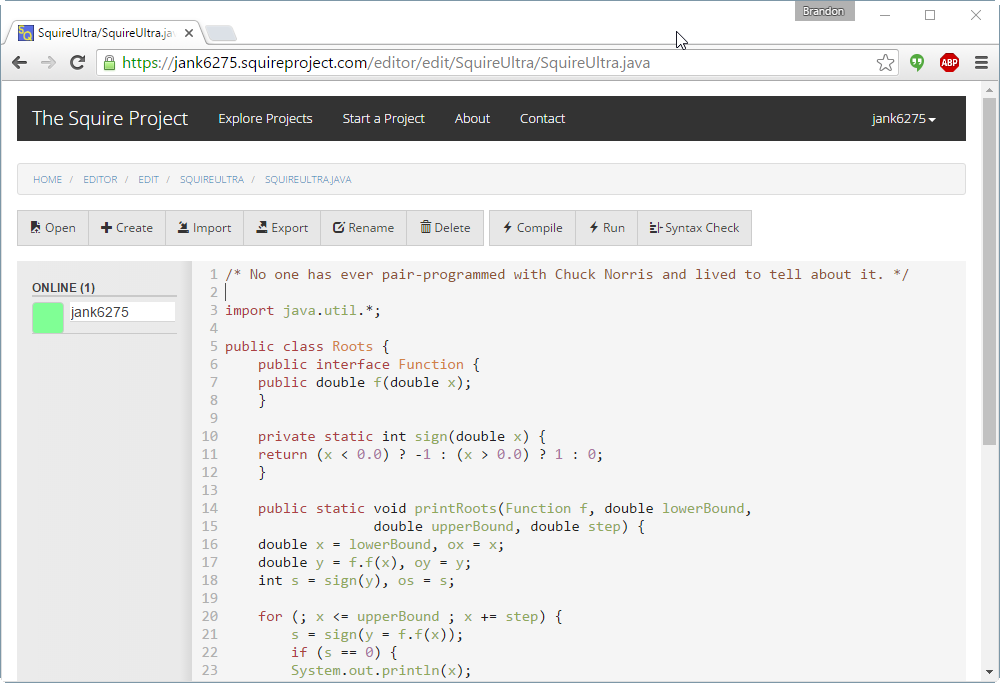
\includegraphics[width=0.9\textwidth]{images/editor}
    \begin{itemize}
        \item Created a new view for project file listing that can be included as a widget on any page. (jank6275)
        \item Created a custom file, project, or user not found page. (jank6275)
        \item Active users, their current line position, and color coding has been fully implemented. (jank6275)
        \item Syntax coloring for Java has been implemented. (jank6275)
        \item Files can now be created and deleted by project members. (jank6275)
        \item Editor was integrated into the new bootstrap format. (jank6275)
        \item Created searchable and orderable project file listing. (jank6275)
        \item Created file location breadcrumb. (jank6275)
        \item File export functionality has been added. (jank6275)
    \end{itemize}
    
\section{Projects Team (boss2849 and brec9824)}
    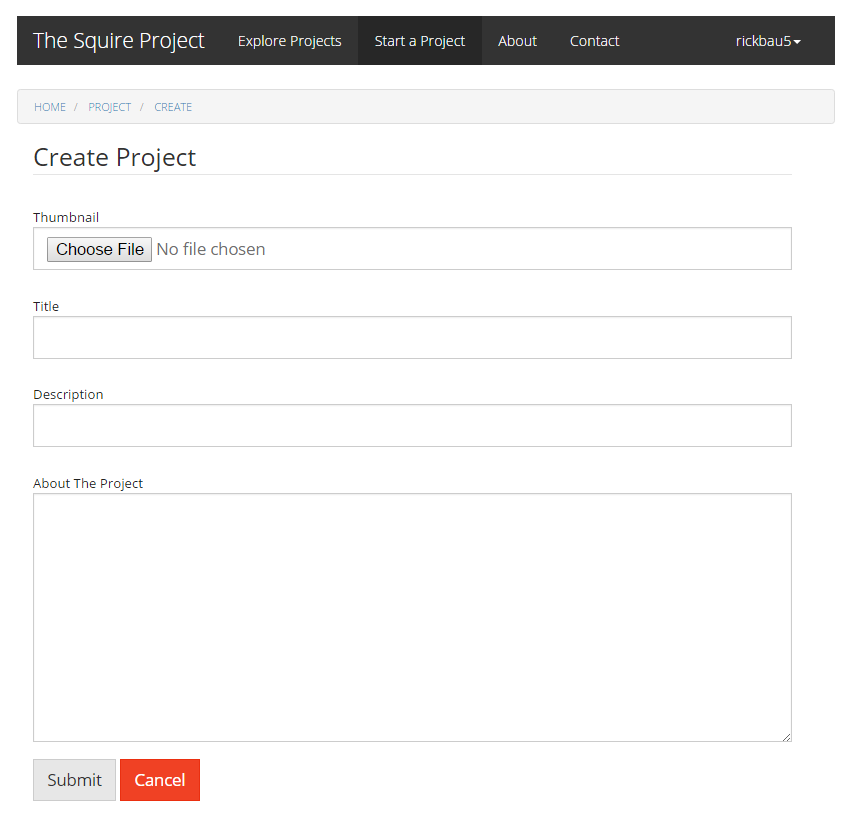
\includegraphics[width=0.9\textwidth]{images/project}
    \begin{itemize}
        \item Start project: Added image upload, title, description, and body for the user to specify when creating a project. (boss2849)
        \item Start project: User must be logged in to start a project. (boss2849)
        \item Start project: Implemented title uniqueness requirement. (boss2849)
        \item Start project: Implemented length constraints on title, description and body as well as verifying an image is uploaded for thumbnail. (boss2849)
        \item Project view: Updated the project view layout to fit the new CSS theme. (brec9824)
        \item Created unit testing for Login, Registration, General permissions, Project creation and viewing. (boss2849)
        \item Updated create project, login, register, and reset forms to all use new css theme. (boss2849)
        \item Project list: Created a new view for the project list. (jank6275)
        \item Project list: Added pagination, only 16 projects are displayed at a time, the rest overflowing to following pages. (boss2849)
        \item Project list: Added sorting, sortable ascending/descending by author, title, and creation/modified dates. (boss2849)
        \item Fixed issues on project list page: Titles and descriptions overflowing. (brec9824)
        \item Fixed issues on project list page: Pictures not scaling correctly. (brec9824)
        \item Fixed issues on project list page: Project thumbnails not of equal size. (brec9824)
        \item Implemented a comments section allowing users the ablity to ask questions about a project. (brec9824)
        \item Comment section: User constraints. (brec9824)
        \item Comment section: Error messages dealing with comments. (brec9824)
        \item Comment section: Edit past comments. (brec9824)
        \item Comment section: Delete past comments. (brec9824)
        \item Comment section: Success messages. (brec9824)
        \item Implemented a project follow allowing users the ablity to follow a project. (brec9824)
        \item Follow project functionality: Follow a project. (brec9824)
        \item Follow project functionality: Unfollow a project. (brec9824)
        \item Follow project functionality: Display follower count for project. (brec9824)
    \end{itemize}

\section{Settings Team (mars2681 and snev7821)}
    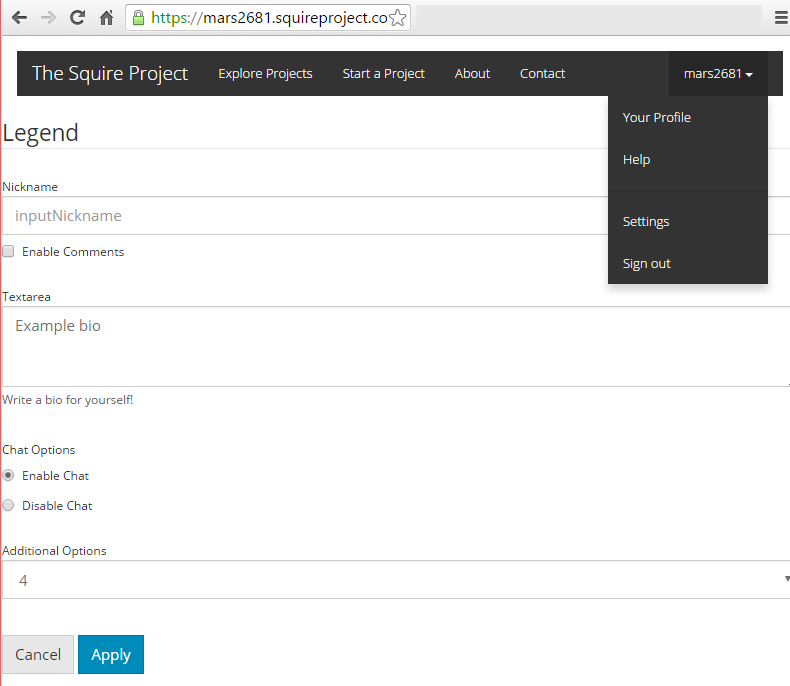
\includegraphics[width=0.9\textwidth]{images/settings}
    \begin{itemize}
        \item Created Settings Controller. (mars2681 and snev7821)
        \item Created Settings Class. (mars2681 and snev7821)
        \item Created Settings Page. (mars2681 and snev7821)
        \item Created Settings Table. (mars2681 and snev7821)
    \end{itemize}

\section{Authentication Team (brec9824)}
    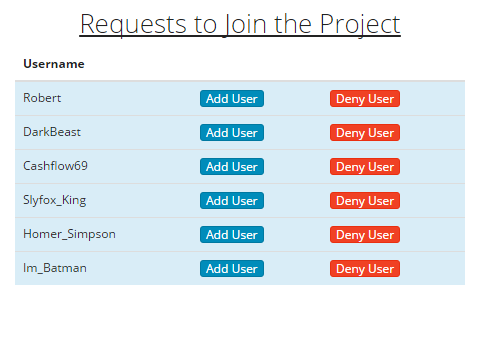
\includegraphics[width=0.9\textwidth]{images/auth}
    \begin{itemize}
        \item Added the ability to login with username or email. (brec9824)
        \item Project Permissions: Request to join (Partial). (brec9824)
        \item Project Permissions: Cancel request. (brec9824)
        \item Project Permissions: Accept request (Partial). (brec9824)
        \item Project Permissions: Deny request (Partial). (brec9824)
    \end{itemize}

\chapter{Unit Testing}
\section{Unit Test Plan}
    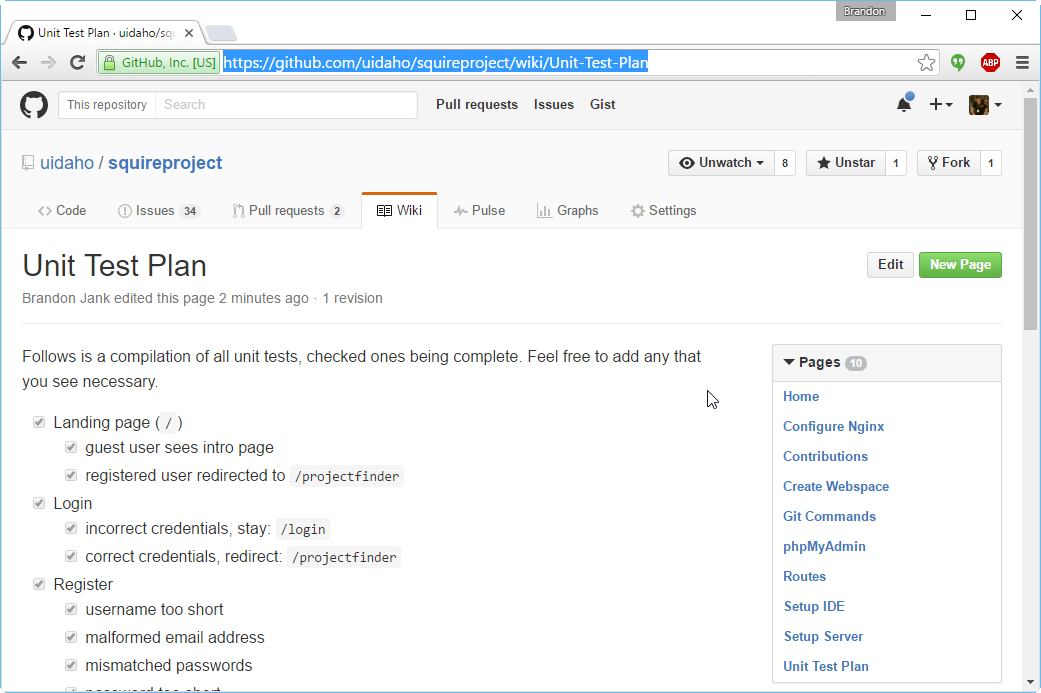
\includegraphics[width=0.9\textwidth]{images/testplan}
    Our unit test plan can be found on the project github wiki at: \url{https://github.com/uidaho/squireproject/wiki/Unit-Test-Plan}

\section{Implemented Unit Tests}
    \begin{itemize}
        \item Unit tests for all methods and user interface elements in the editor have been implemented. (jank6275)
        \item Login: Deny invalid credentials. (boss2849)
        \item Login: Accept valid credentials and redirect. (boss2849)
        \item Project comments: Auth/non-auth users view. (brec9824)
        \item Project comments: Creating a comment. (brec9824)
        \item Project comments: Editing a comment. (brec9824)
        \item Project comments: Deleting a comment. (brec9824)
        \item Project following: Tests auth/non-auth users view. (brec9824)
        \item Project following: Following a project. (brec9824)
        \item Project following: Users view after someone else follows the project. (brec9824)
        \item Project following: Unfollowing a project. (brec9824)
        \item Project creation: Visit as guest. (boss2849)
        \item Project creation: Invalid title. (boss2849)
        \item Project creation: Invalid description. (boss2849)
        \item Project creation: Invalid body. (boss2849)
        \item Project creation: Invalid image. (boss2849)
        \item Project creation: Create valid project. (boss2849)
        \item Project page test: Attempt delete project using direct link. (boss2849)
        \item Project page test: Attempt delete project as non-owner. (boss2849)
        \item Project page test: Delete a valid proejct. (boss2849)
        \item Registration: Invalid username. (boss2849)
        \item Registration: Invald email address. (boss2849)
        \item Registration: Mismatched passwords. (boss2849)
        \item Registration: Invalid password. (boss2849)
        \item Registration: Valid input. (boss2849)
    \end{itemize}

\end{document}